\documentclass[12pt, demo]{article}
\usepackage[margin=1in]{geometry}
\usepackage{pythontex}
\usepackage{tabularx}
\usepackage{graphicx}
\usepackage{titling}
\usepackage{amsmath}
\usepackage{ragged2e}

\title{Using Machine Learning to Predict Typing Speed\vspace{-3em}}
\author{jjr117}
\date{}

\newcommand{\code}[1]{\texttt{#1}}

\newenvironment{textexamples}
  {\medskip\par\setlength{\parindent}{0pt}}
  {\par\medskip}

\graphicspath{{assets/}}

\begin{document}

\maketitle

\section*{Introduction}

One of my hobbies is competitive typing, where I compete with my friends to type a text as quickly as possible. I often use a website called TypeRacer, where your goal is to drive a racecar to the finish line, and the position of your racecar is determined by how many words you've typed correctly in the quote:

\begin{figure}[hbt!]
	\caption{A screenshot of a typing competition on the website \textit{TypeRacer}}
	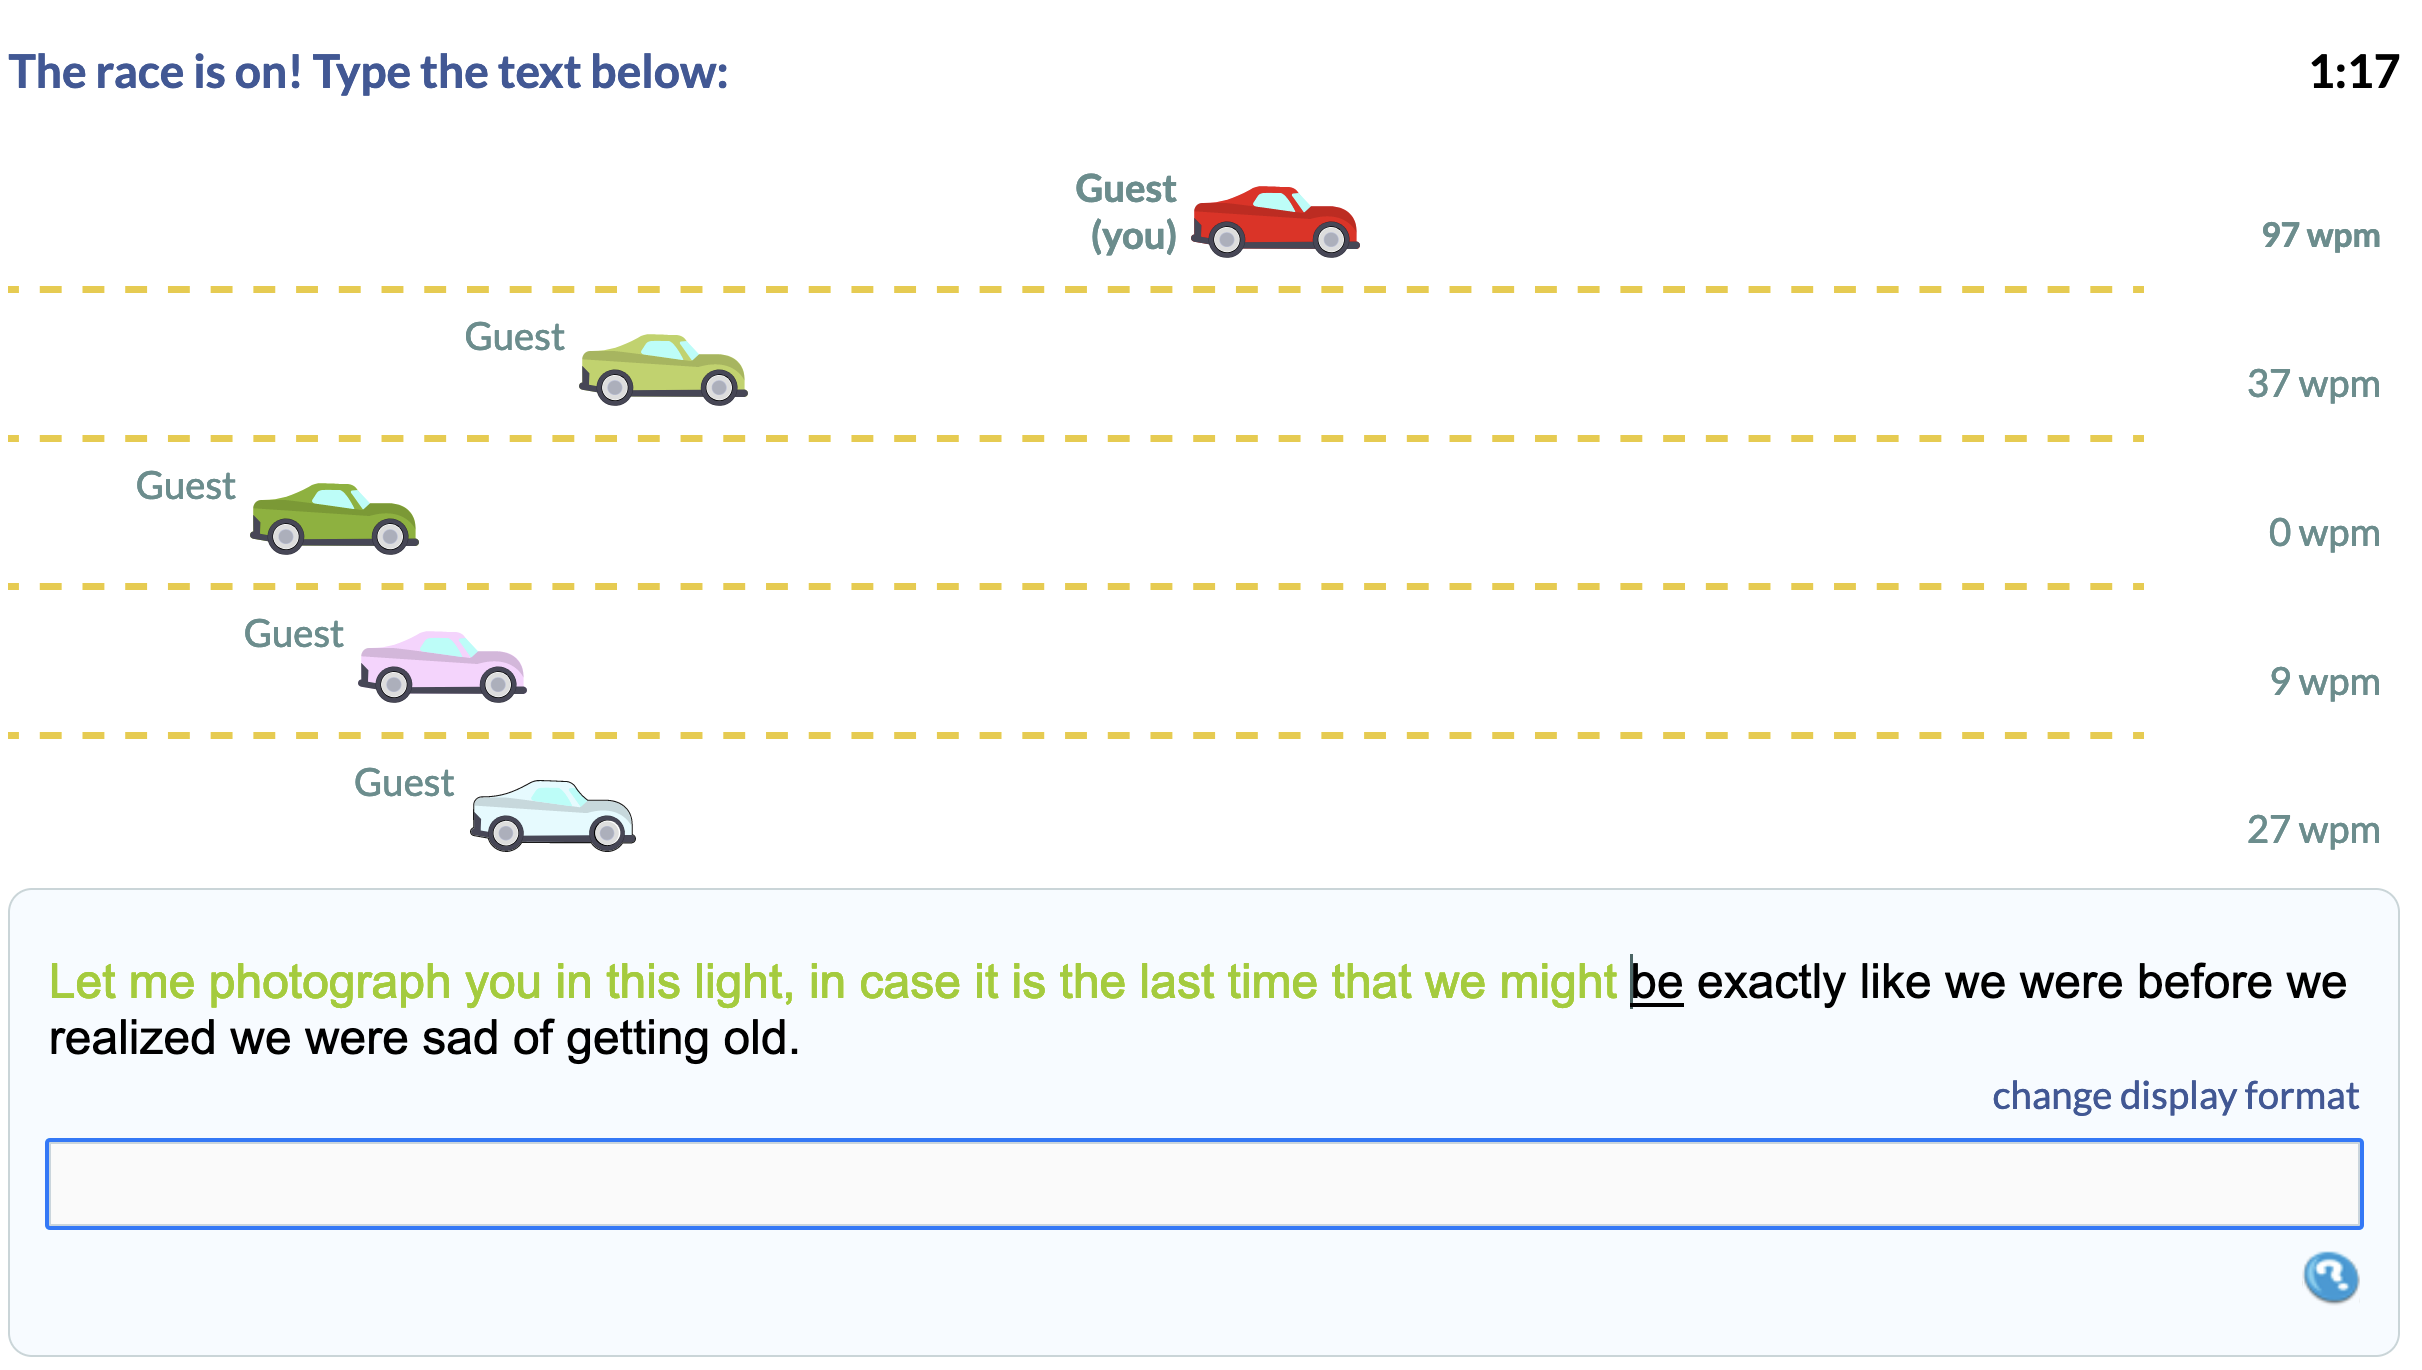
\includegraphics[width=\textwidth]{typeracer.png}
\end{figure}

Your score is a measurement of your average typing speed at the end of the race. Typing speed is measured in the units "words per minute" ("wpm" for short), and each word is defined as five characters.

In TypeRacer, your typing speed determines the types of texts you'll be presented with: a lower typing speed gives you easier texts, while a higher typing speed gives you more difficult texts:

\begin{figure}[hbt!]
	\caption{Two different possible texts in TypeRacer. On the left, an easy text, and on the right, a more difficult text.}
	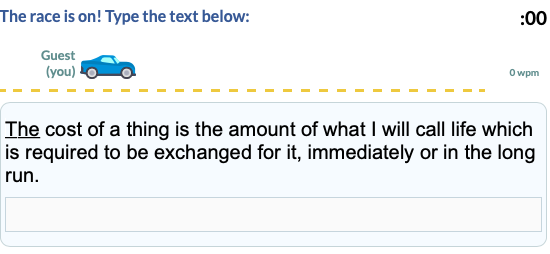
\includegraphics[width=0.5\textwidth]{easy-text.png}
	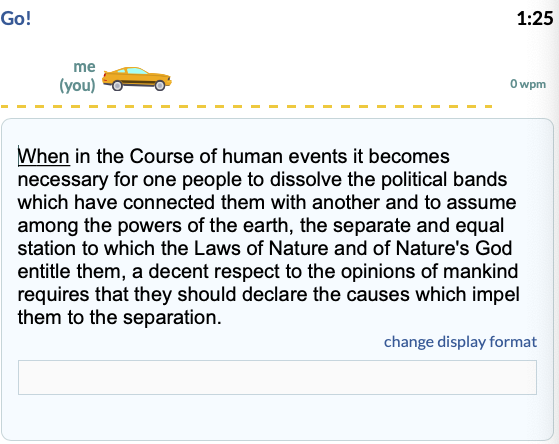
\includegraphics[width=0.5\textwidth]{hard-text.png}
\end{figure}


However, not all texts are created equal. Some texts are harder to type than others, whether it's from having longer, more complex words, frequent capital letters, numbers, etc.

Predicting the difficulty of a text is useful. For example, the typing site that I practice on, TypeRacer, will display different sets of texts depending . For example, these are two quotes that can appear in a TypeRacer race:


Even though Quote 1 is shorter than Quote 2, the difficult word at the start of Quote 1 makes it significantly more difficult to type.

Currently, the way TypeRacer classifies the difficulty of a newly added quote is through . Each player has an average typing speed that is calculated based on their best scores for each quote, and if the

At first, I considered using the length of the text might be to use the length of the text in determining its difficulty. While this works for the two texts shown in Figure 1, it's not a flawless approach. For example, the following two texts are possible texts you can encounter in TypeRacer:

\begin{textexamples}
	\textbf{Text 1}: Supercalifragilisticexpialidocious is Vielle's favorite word to type on TypeRacer.
	\textbf{Text 2}: For someone who was never meant for this world, I must confess I'm suddenly having a hard time leaving it.
\end{textexamples}

Even though Text 1 has fewer characters than Text 2, it is still considerably more difficult to type because of the complex first word.

, but there are many more characteristics of words that affect the speed at which they are typed. For example, one of these characteristics is the fingers you use to type the word.

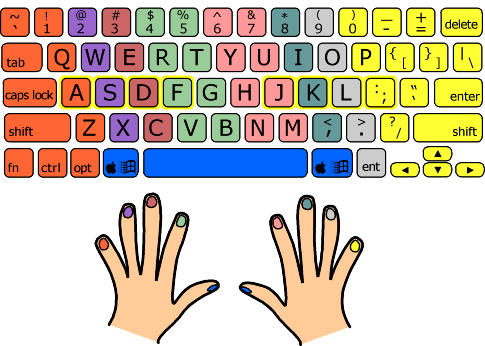
\includegraphics{finger-map.png}

Using this standard finger map, when typing the word \texttt{mummy} on the QWERTY keyboard, you would exclusively use your right index finger to type the entire word, making it significantly slower to type compared to a word like \texttt{there}, which doesn't involve using the same finger to type two consecutive letters.

\begin{textexamples}
\end{textexamples}

The characteristics of how difficult a word is to type extends beyond these two examples, and each characteristic has a different amount of influence on how quickly I type the word. In order to determine the significance of these various characteristics in the difficulty of a word, machine learning can be applied.

\section*{Gathering Data}

In order to create a machine learning algorithm that predicts how fast I can type a certain text based on the text features, we need to collect a large amount of data that includes various texts and the speed at which I type them. Luckily, I've been using TypeRacer for over 5 years now, and over these 5 years I've typed over 8000 texts on my account.

I created a program that automatically scrapes the race data from all my 8000 races and saves them into a file.

% TODO: Why WPM Ratio?

\section*{Analyzing Data}

Thus, to take into consideration the gradual increase in my typing speed overtime, the typing speed of a word should be measured relative to my average speed at the time.

After analyzing the data, I noticed some outliers in the data set. Occasionally, I take a short breather in the middle of a typing race if I'm making too many mistakes, and this is reflected in some of the data as it causes my algorithm to calculate abnormally low speeds for some words. To counter this problem, I decided to take the median of the wpm ratios, as it wouldn't be as affected by outlier data compared to the mean.

\section*{Predicting Typing Speed}

The WPM Ratio of a word depends on various features of the word, such as the length of the word and the amount of capital letters in the word.

For example, if the typing speed of a word was linearly proportional to its length, then our predictive function might look like the following:
\begin{align}
	\text{WPM Ratio} = w_{\text{word length}} * (\text{word length}) + Bias
\end{align}

This equation resembles the typical linear equation $y = mx + b$, where $w_{\text{word length}}$ represents the slope, or in other words, the amount that the WPM Ratio increases or decreases by when the word length is increased by 1.

However, when we plot the graph of word length against WPM Ratio, we get the following figure:

\begin{figure}
	\caption{Word Length vs. WPM Ratio}
	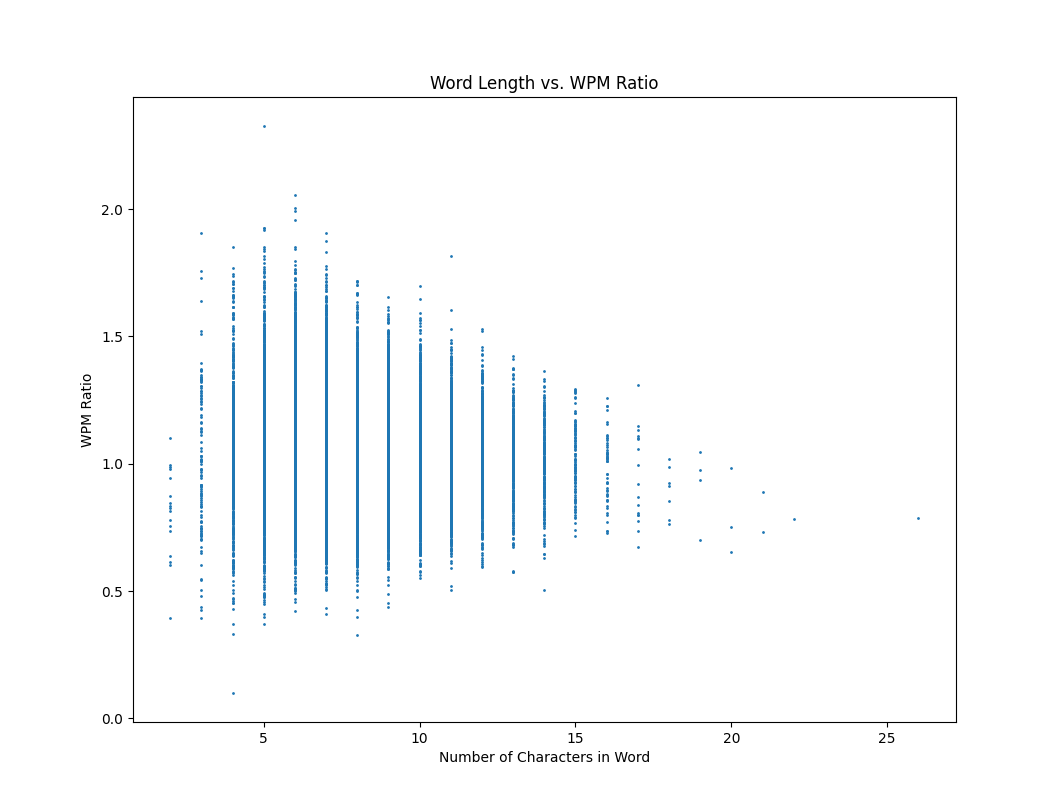
\includegraphics{word-length-vs-wpm.png}
\end{figure}

The graph indicates that longer words typically have lower WPM Ratios, but the range of WPM ratios for shorter words is much larger. If we filter out words that have a WPM ratio lower than 0.5, we can understand why:

% \begin{noindent}
\begin{pycode}
word_stats = [
	word_stat.strip().split('|') for word_stat in """
		"If |0.4905423436151009
		L.A. |0.48295763254168533
		DOS |0.46217555276196115
		"No |0.428899294475664
		'How |0.3993690501499697
		UBS |0.4679134219795311
		GROW |0.4646458701500651
		Six? |0.48037553838088465
	""".strip().splitlines()
]

def get_table():
	table = """
		\\begin{center}
		\\noindent
		\\begin{tabularx}{
			0.5\\linewidth
		}{|X|X|}
		\\hline
		Word (wrapped in ``'') & WPM Ratio
	"""
	for word_stat in word_stats:
		table += f"""
			\\\\\\hline
			``\\code{{{word_stat[0]}}}'' & {"%.3f" % float(word_stat[1])}
		"""
	table += """
		\\\\\\hline
		\\end{tabularx}
		\\end{center}
	"""
	return table
\end{pycode}
% \end{noindent}

\py{get_table()}

Even though these words are short, they contain capital letters and keys that need you to press the Shift key to type (\code{"} and \code{?}). This makes the word substantially slower to type, and isn't accounted for in Equation x.

Our function must take into account various features of the word that would affect typing speed. Some features, like the number of capital letters, will influence the word's typing speed more compared to other features, like whether the word starts with a vowel or a consonant.

To account for the different influences of different features, we need to assign a different weight to each of them in our equation, which gives us an equation similar to the following:

\begin{align*}
	f(\text{word}) = w_1 * (\text{Feature 1}) + w_2 * (\text{Feature 2}) + ... + \text{Bias}
\end{align*}

For example, if the only two features that influence the difficulty of a are the length of the word and the number of capital letters in the word, then the equation would become:

\begin{align*}
	\text{Difficulty} = w_{\text{word length}} * (\text{word length}) + w_{\text{capital letters}} * (\text{\# of capital letters}) + \text{Bias}
\end{align*}

% where $w_{\text{word_length}}$ isn't necessarily the same as $w_{\text{capital letters}}$.

How do we find the optimal values of $w_{\text{feature}~i}$ that will give us the most accurate function for predicting a word's WPM ratio? This is where machine learning comes in.

\section*{Machine Learning}

\subsection*{The Cost Function}

The cost function will inform our machine learning algorithm how accurate its weights are, and more importantly, how to adjust its weights in order to reduce the cost.

One popular cost function used in machine learning is the MSE (Mean Squared Error). This function defines the cost as the squares of the difference between the actual data ($y_i$) and the predicted data ($f(x_i)$):
\begin{align*}
	C(f) & = \frac{1}{N}\big[(y_1 - f(x_1))^2 + (y_2 - f(x_2))^2 + ... + (y_n - f(x_n))^2]
	\\
	C(f) & = \frac{1}{N} \sum_{i=1}^{n} (y_i - f(x_i))^2
\end{align*}

To visualize this cost function, I've plotted the below data for a small set of words that have a clear correlation between word length and WPM Ratio:

% \begin{noindent}
\begin{pycode}
word_data = [
	['month.', 6, 1.8523997581589209],
	['should ', 7, 1.7302841332533008],
	['meaning.', 8, 1.614390135538142],
	['singing. ', 9, 1.5007211799003408],
	['thoughts. ', 10, 1.448833713008257],
	['standpoint ', 11, 1.3051500032628751],
]

def get_table_row(row_index: int):
	return f"""
		\\\\\\hline
		``{word_data[row_index][0]}'' &
		{word_data[row_index][1]} &
		{"%.3f" % word_data[row_index][2]}
	"""
def f3f(number):
	return "%.3f" % number
\end{pycode}
% \end{noindent}

\begin{tabularx}{\linewidth}{|X|X|X|}
	\hline
	Word        &
	Word Length &
	WPM Ratio

	\py{get_table_row(0)}
	\py{get_table_row(1)}
	\py{get_table_row(2)}
	\py{get_table_row(3)}
	\py{get_table_row(4)}
	\py{get_table_row(5)}

	\\\hline
\end{tabularx}

A visual example of this cost function would look like:

\includegraphics{mse-cost.png}

The goal of our machine learning algorithm is to minimize this function: to find a set of weights for our prediction function $f$ such that $C(f)$ is as low as possible. A popular method for minimizing cost is by using gradient descent.

\subsection*{Gradient Descent}

Gradient descent involves using the derivative of a function to find a function's local minimum. In our case, we need to find the local minimum of our cost function, $C$.

Let's consider the case where our prediction function $f$ is correlated with only one weight, the text length.  For convenience, we'll denote "word $i$" as $x_i$, "text length of word $i$" as $l_i$, and "Bias" as $b$:
\begin{align}
	f(x_i) = w_1 * l_i + b
\end{align}

For this definition of $f$, our cost function would look like the following:
\begin{align}
	C(f) & = \frac{1}{N} \sum_{i=1}^{n} (y_i - f(x_i))^2
	\\
	C(f) & = \frac{1}{N} \sum_{i=1}^{n} (y_i - w_1 * l_i - b)^2
\end{align}

\begin{itemize}
	\item Whether the word is common (1 if the word is included within the top 1000 most common English words, and 0 otherwise).
	\item The number of capital letters in the word.
	\item The number of characters in the word.
	\item The number of sets of "double letters" in the word. For example, the word "sheep" has 1 set of double letters, and the word "bittersweet" has two sets of double letters.
	\item The number of letters in the home row of the keyboard (the row with the letters "asdf" on the QWERTY layout).
	\item The number of letters that require pressing the "Shift" key to type.
	\item The amount of times the same finger is used to type consecutive letters in the word. For example, the word "mummy" requires using the right index finger five times in a row on a QWERTY layout.
	\item The number of letters typed with the left hand.
	\item The number of letters typed with the right hand.
\end{itemize}

\textbf{Note:} The data in the following tables might not match with the data you'd expect on a QWERTY layout, and that's because when analyzing my typing data, I based it off the keyboard layout that I use—the Programmer Dvorak layout—which looks like this:

% \begin{noindent}
\begin{pycode}
word1 = {"word":"profession ","medianWpm":154.134295227525,"isWordCommon":0,"numCapitalLetters":0,"numConsecutiveFingers":1,"numDoubleLetters":1,"numHomeRowLetters":7,"numLeftHandLetters":5,"numNumbers":0,"numRightHandLetters":5,"numShiftedLetters":0,"wordLength":11}

word2 = {"word":"Table, ","medianWpm":136.84411614875188,"isWordCommon":1,"numCapitalLetters":1,"numConsecutiveFingers":0,"numDoubleLetters":0,"numHomeRowLetters":2,"numLeftHandLetters":3,"numNumbers":0,"numRightHandLetters":3,"numShiftedLetters":1,"wordLength":7}

word3 = {"word":"1950s, ","medianWpm":81.3953488372093,"isWordCommon":0,"numCapitalLetters":0,"numConsecutiveFingers":0,"numDoubleLetters":0,"numHomeRowLetters":1,"numLeftHandLetters":4,"numNumbers":4,"numRightHandLetters":2,"numShiftedLetters":4,"wordLength":7}

def get_table_1_row(w):
	return f"""
		\\\\\\hline
		"{w['word']}" &
		{w['wordLength']} &
		{w['numCapitalLetters']} &
		{w['numConsecutiveFingers']} &
		{w['numDoubleLetters']} &
		{w['numHomeRowLetters']}
	"""

def get_table_2_row(w):
	return f"""
		\\\\\\hline
		"{w['word']}" &
		{w['numLeftHandLetters']} &
		{w['numRightHandLetters']} &
		{w['numNumbers']} &
		{w['numShiftedLetters']} &
		{w['isWordCommon']} &
		{"%.2f" % w['medianWpm']}
	"""
\end{pycode}
% \end{noindent}

\begin{table}[hbt!]
	\caption{Three examples of features in words}
	\begin{tabularx}{\linewidth}{|
			p{70pt}|
			>{\RaggedRight}X|
			>{\RaggedRight}X|
			>{\RaggedRight}X|
			>{\RaggedRight}X|
			>{\RaggedRight}X|
			>{\RaggedRight}X|
		}
		\hline

		Word                               &
		\# of Characters                   &
		\# of Capitals                     &
		\# of Same-Finger Consecutive Keys &
		\# of Double Letters               &
		\# of Home Row Letters

		\py{get_table_1_row(word1)}
		\py{get_table_1_row(word2)}
		\py{get_table_1_row(word3)}
		\\\hline
	\end{tabularx}

	\begin{tabularx}{\linewidth}{|
			p{70pt}|
			>{\RaggedRight}X|
			>{\RaggedRight}X|
			>{\RaggedRight}X|
			>{\RaggedRight}X|
			>{\RaggedRight}X|
			>{\RaggedRight}X|
			>{\RaggedRight}X|
		}
		\hline

		Word                          &
		\# of Left Hand Letters       &
		\# of Right Hand Letters      &
		\# of Numbers                 &
		\# of Letters Requiring Shift &
		Is word common?               &
		Median WPM

		\py{get_table_2_row(word1)}
		\py{get_table_2_row(word2)}
		\py{get_table_2_row(word3)}
		\\\hline
	\end{tabularx}
\end{table}


\begin{figure}[hbt!]
	\caption{The Programmer Dvorak Keyboard Layout}
	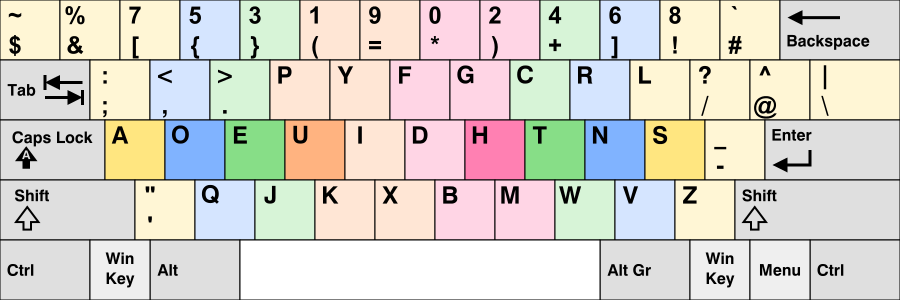
\includegraphics[width=\textwidth]{programmer-dvorak.png}
\end{figure}

\end{document}